\chapter{Validation of the simulation}
\label{appendix:SimulationVal}

\section{Beam profiles}

The simulation needs as one input the position and width of the particle gun. It has to be placed in x, y directions such that the beam sizes of the experiment are modeled and in order to garanty that the same cells of the detector are hit in the simulation as in data. Otherwise, dead and noisy channels could bias the comparison between data and simulation. In the z direction, the beam gun needs to be put as close as possible of the detector to avoid beam broadening by scatering on air molecules.

The best method to estimate the beam profile for data would be to analyse the beam profile provided by the wired chambers. Unfortunately, this data is not available for this analysis. As a work-around, the mean and RMS of the center of gravity distributions in x and y are used to estimate the beam size instead. This does not reflect the true positions since both positions are biased by dead and noisy channels. This has been done for electrons runs as well as for pions runs for each energies. No significant differences in beam profile is visible on a run-by-run basis. The muon beam is simulated by a plane square distribution with a half width of 20 cm. The center of gravity is calculated as the following:

\begin{equation}
  CoG_x [mm] = \frac{\Sigma_i E_i x_i}{\Sigma_i E_i} \quad \text{and} \quad CoG_y [mm] = \frac{\Sigma_i E_i y_i}{\Sigma_i E_i}
\end{equation}

\noindent with $E_i$ the energy of the i-th hit and $x_i$ and $y_i$ the x and y position of the i-th hit.

Figures \ref{fig:BPe} show the beam profiles in the x and y directions for data and simulation for 10 GeV and 50 GeV electrons. The aggrement look much better for 10 GeV than for 50 GeV, this may be due to contamination from lower energy electrons. Moreover, at higher energy, the beam looks less gaussian-like and the shape in simulation can't be simulated correctly. Figures \ref{fig:BPpi} show the beam profiles in the x and y direction for data and simulation for 10 GeV and 90 GeV pions. The aggrement looks quite good for both energies in the x direction, only a slight difference is visible on the y direction but should have not much impact.

\begin{figure}[htbp!]
  \centering
  \begin{subfigure}[t]{0.49\textwidth}
    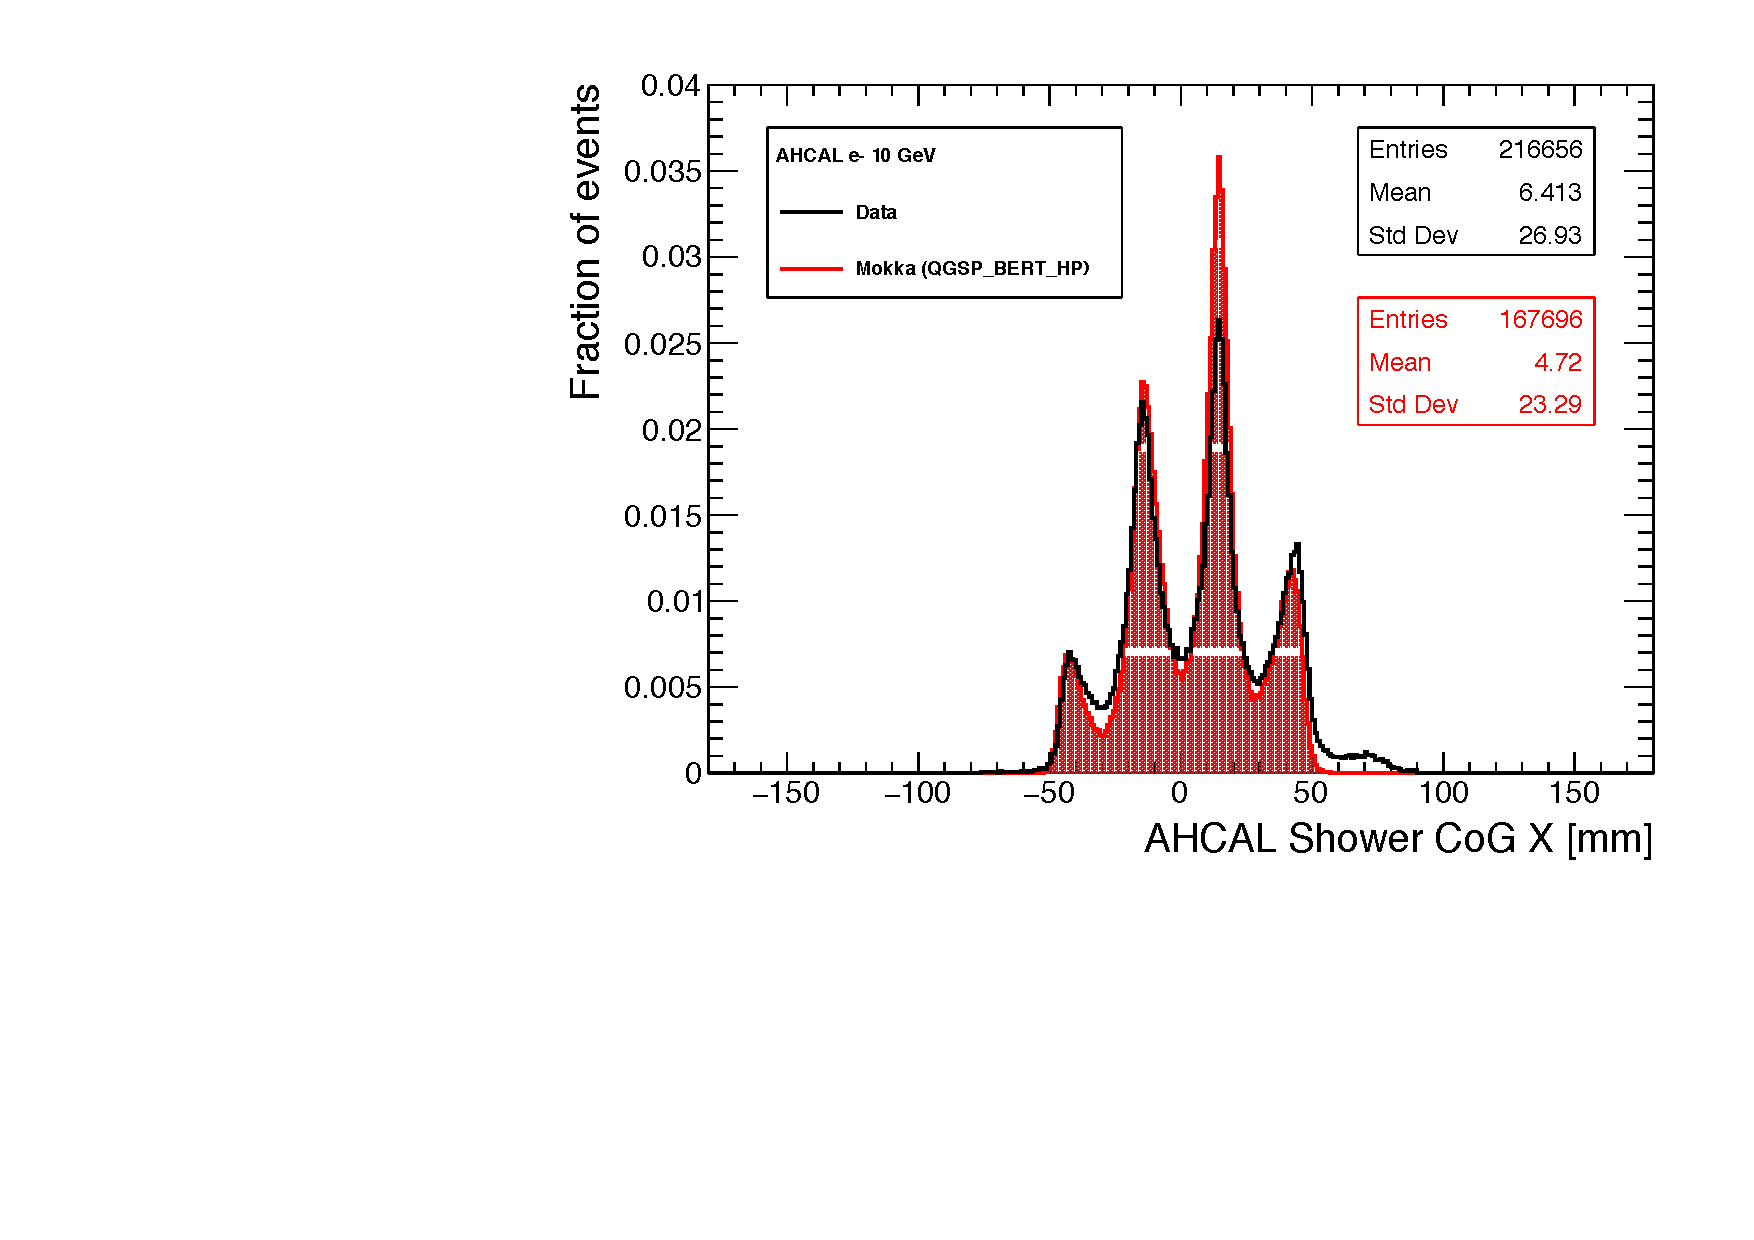
\includegraphics[width=1.\linewidth]{chap5/fig_AHCAL_Timing/Electrons/Run24542_CoGX_AHCAL_10GeV_Comparison.pdf}
    \caption{10 GeV.} \label{fig:e10GeVX}
  \end{subfigure}
  \hfill
  \begin{subfigure}[t]{0.49\textwidth}
    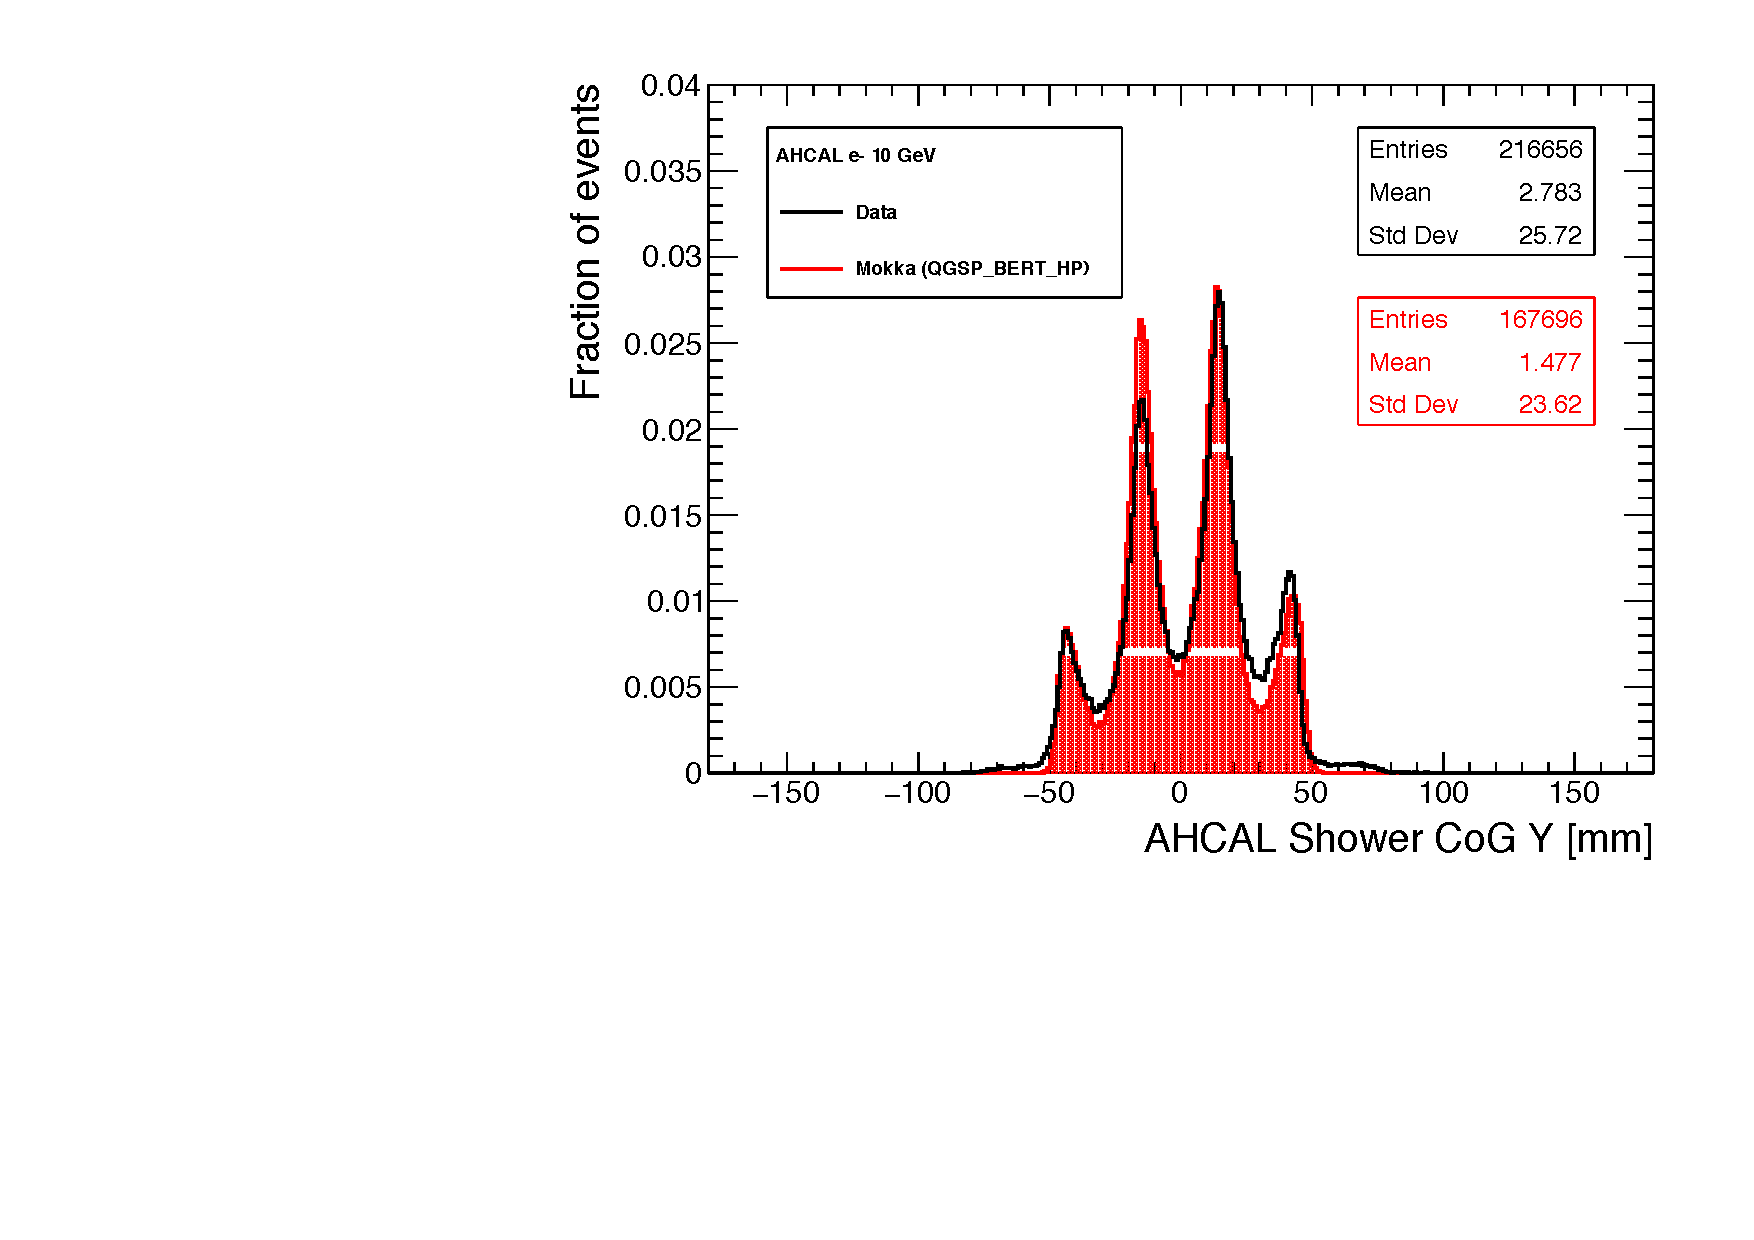
\includegraphics[width=1.\linewidth]{chap5/fig_AHCAL_Timing/Electrons/Run24542_CoGY_AHCAL_10GeV_Comparison.pdf}
    \caption{10 GeV.} \label{fig:e10GeVY}
  \end{subfigure}
  \hfill
  \begin{subfigure}[t]{0.49\textwidth}
    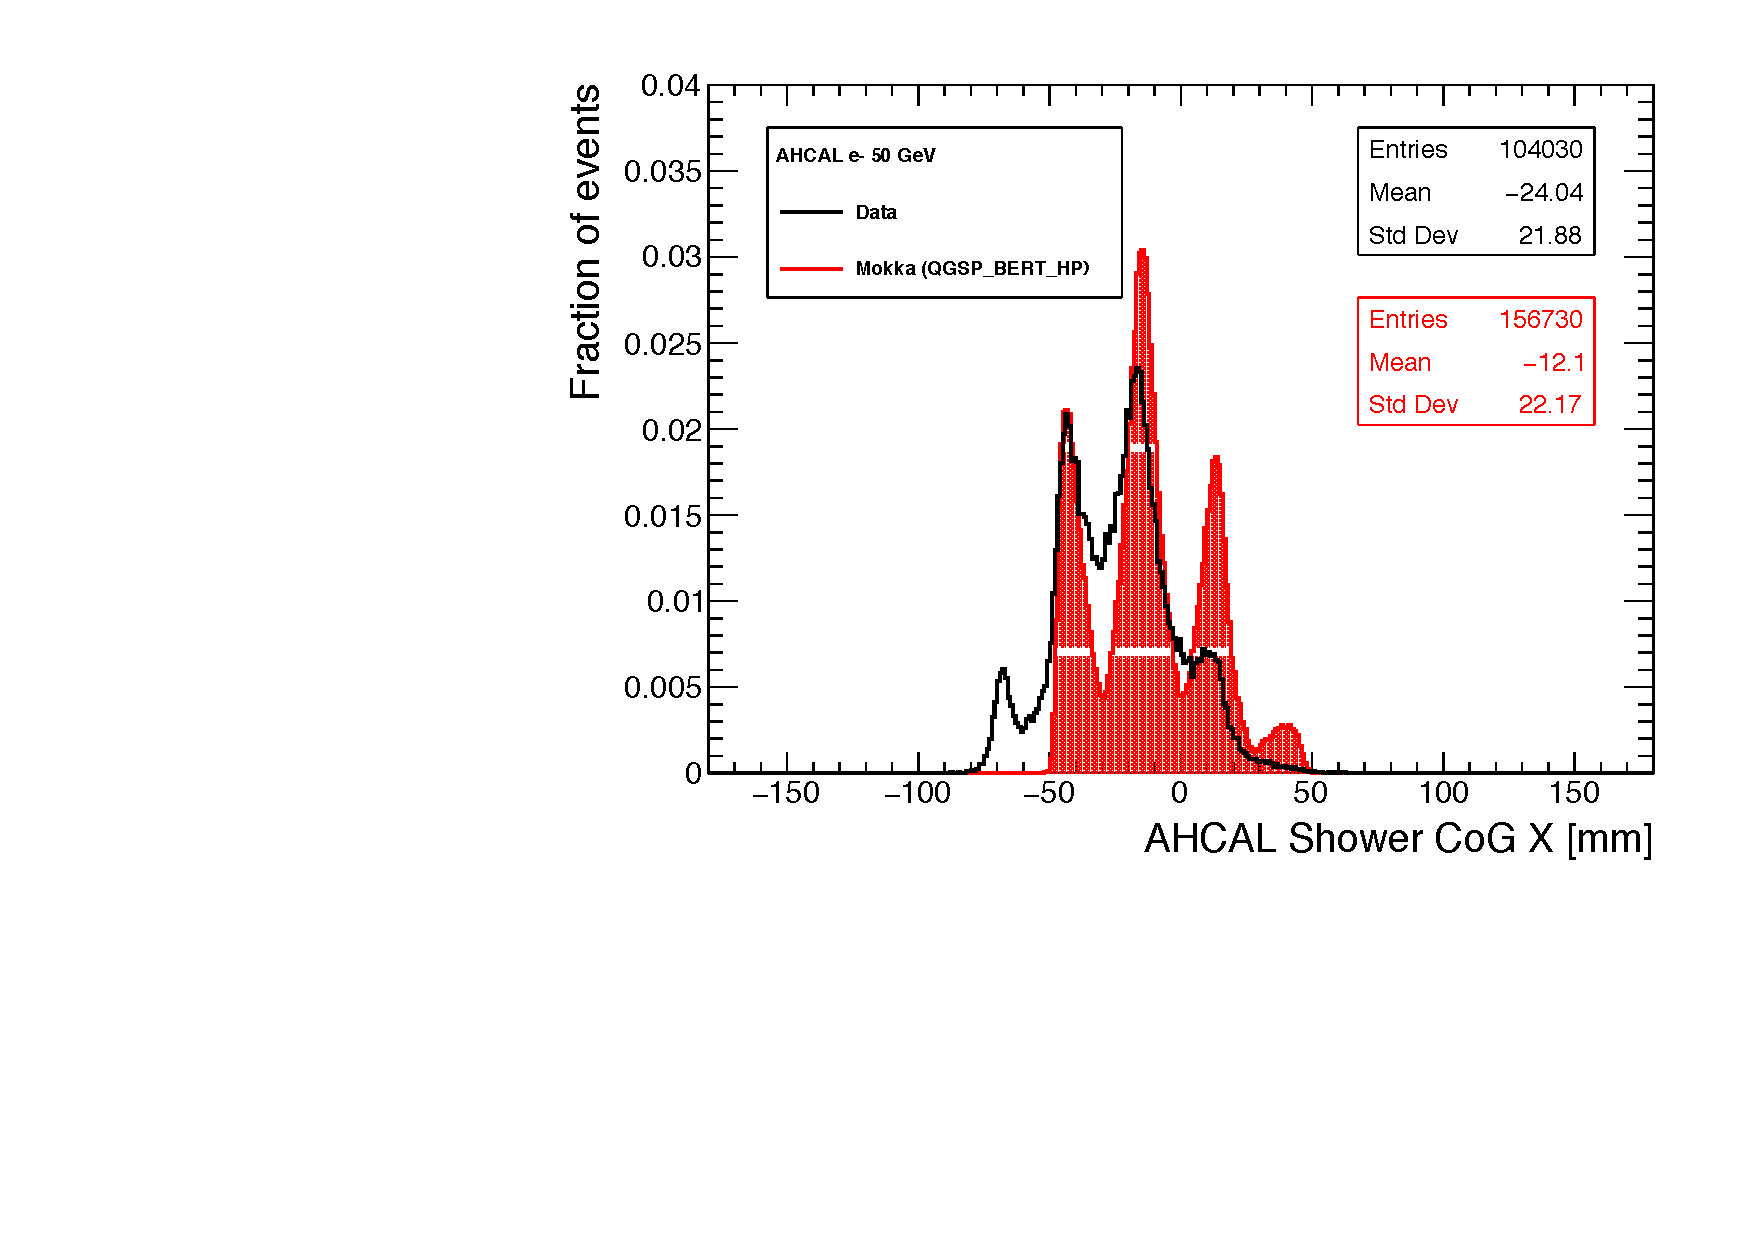
\includegraphics[width=1.\linewidth]{chap5/fig_AHCAL_Timing/Electrons/Run24405_CoGX_AHCAL_50GeV_Comparison.pdf}
    \caption{50 GeV.} \label{fig:e50GeVX}
  \end{subfigure}
  \hfill
  \begin{subfigure}[t]{0.49\textwidth}
    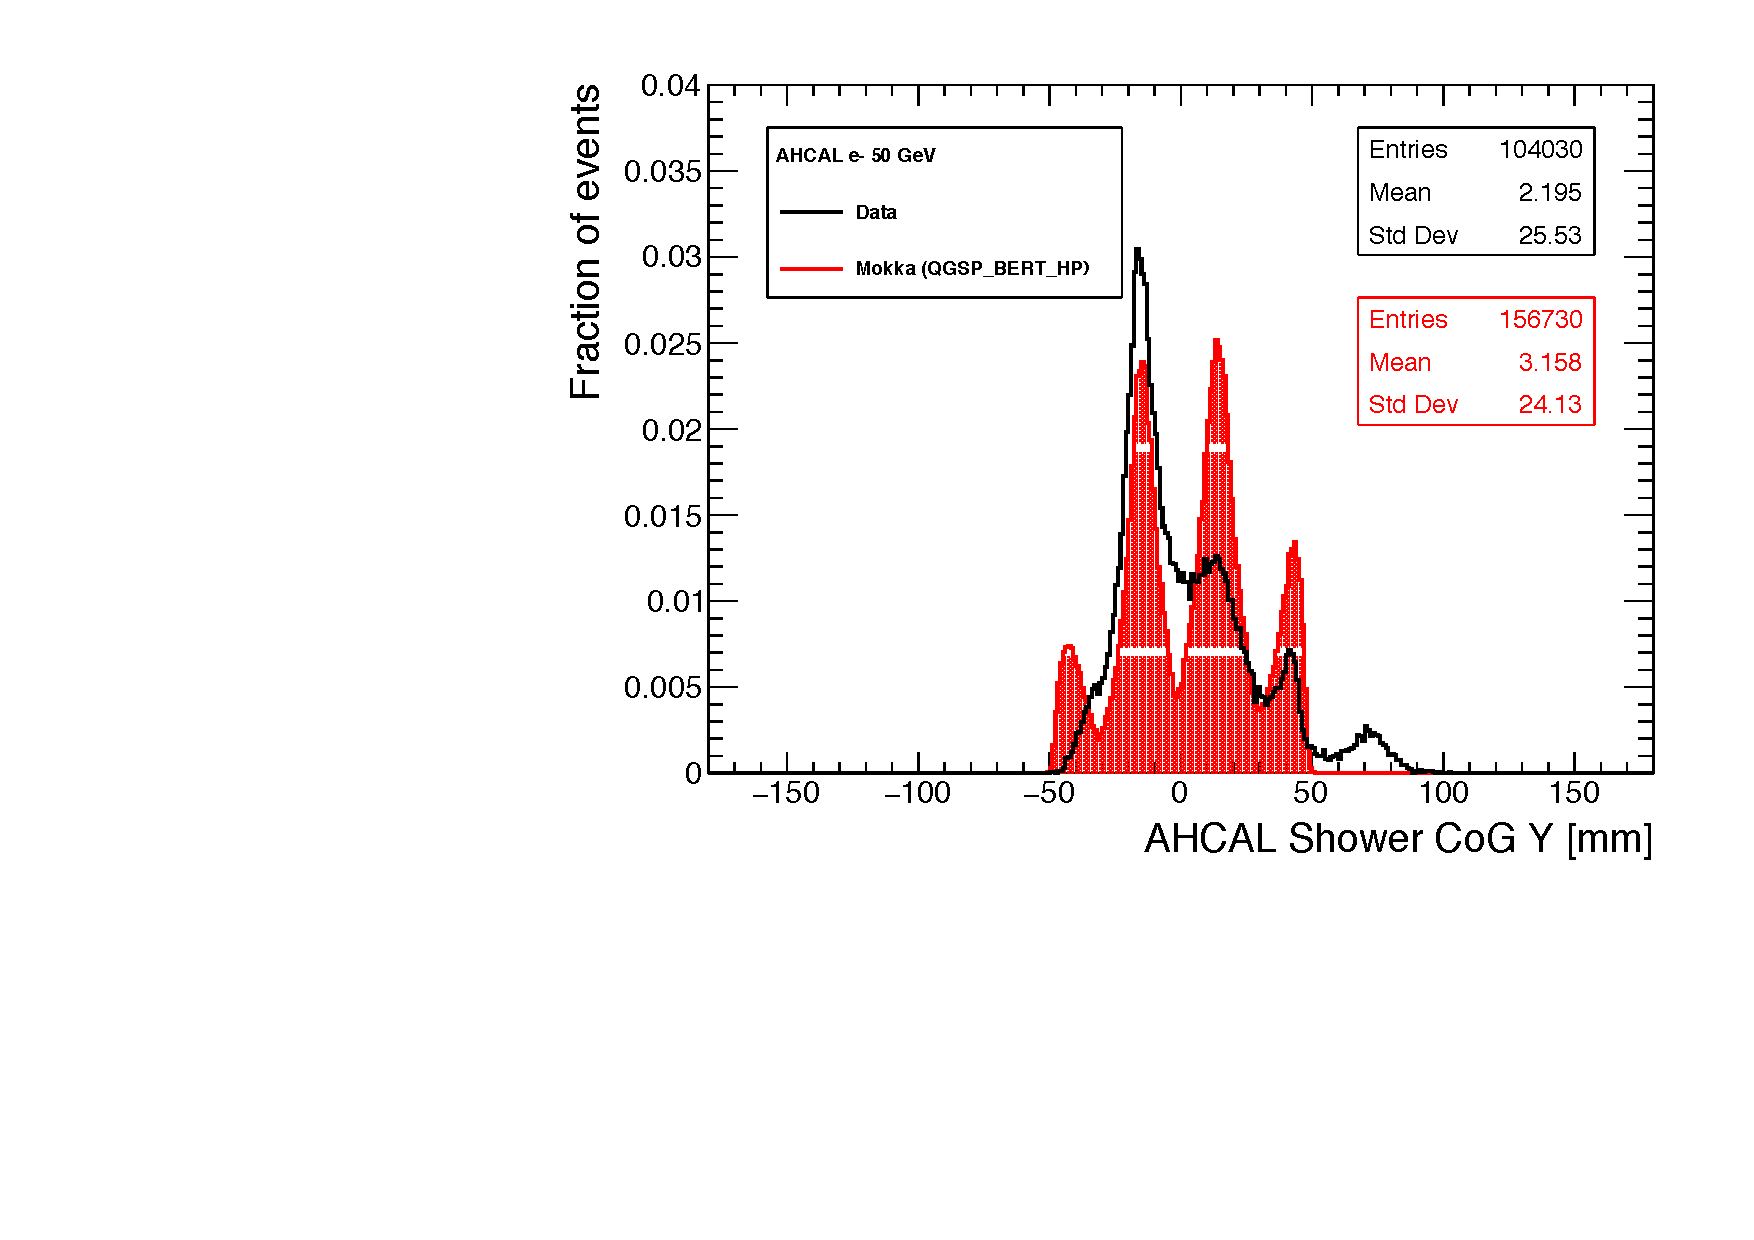
\includegraphics[width=1.\linewidth]{chap5/fig_AHCAL_Timing/Electrons/Run24405_CoGY_AHCAL_50GeV_Comparison.pdf}
    \caption{50 GeV.} \label{fig:e50GeVY}
  \end{subfigure}
  \caption{Beam profiles for 10 GeV and 50 GeV electrons for data and simulation in the x and y directions.}
  \label{fig:BPe}
\end{figure}

\begin{figure}[htbp!]
  \centering
  \begin{subfigure}[t]{0.49\textwidth}
    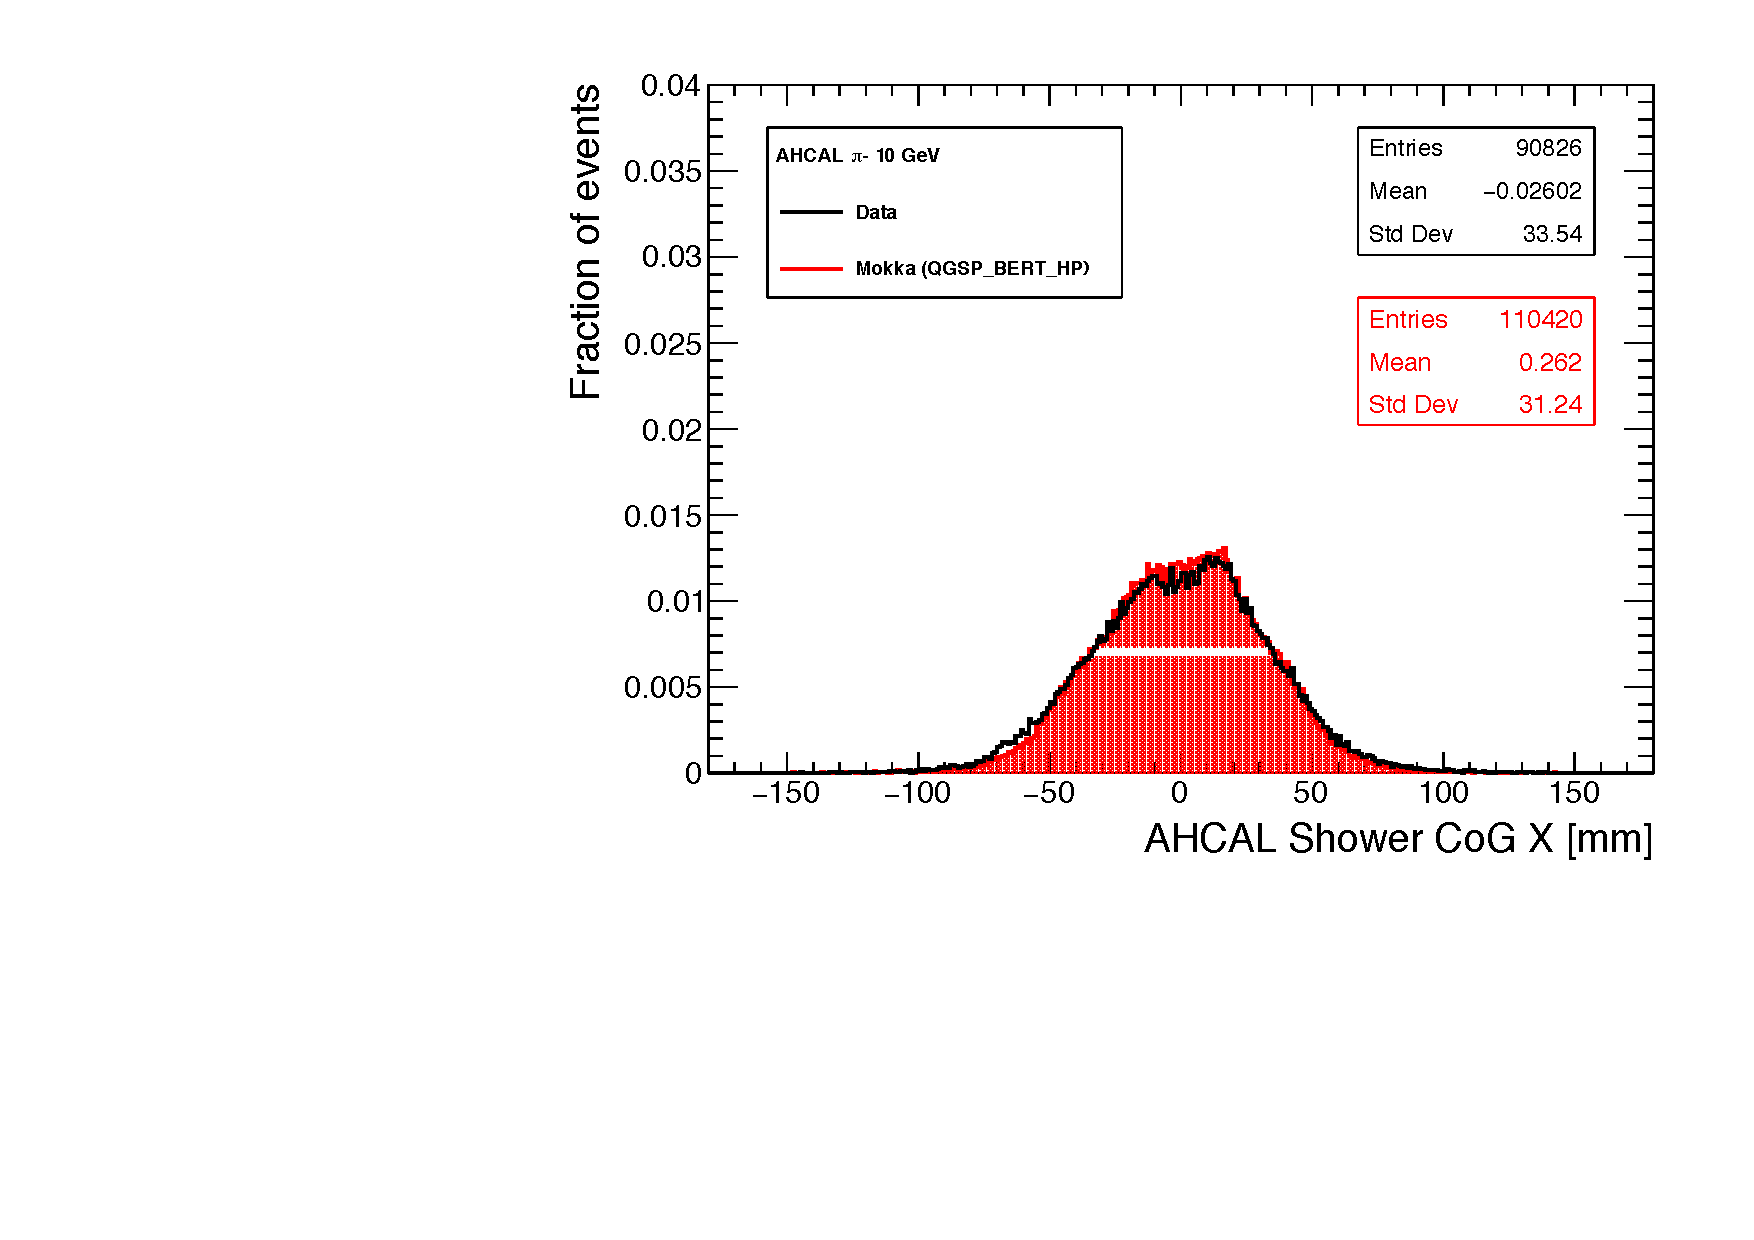
\includegraphics[width=1.\linewidth]{chap5/fig_AHCAL_Timing/Pions/Run24306_CoGX_AHCAL_10GeV_Comparison.pdf}
    \caption{10 GeV.} \label{fig:pi10GeVX}
  \end{subfigure}
  \hfill
  \begin{subfigure}[t]{0.49\textwidth}
    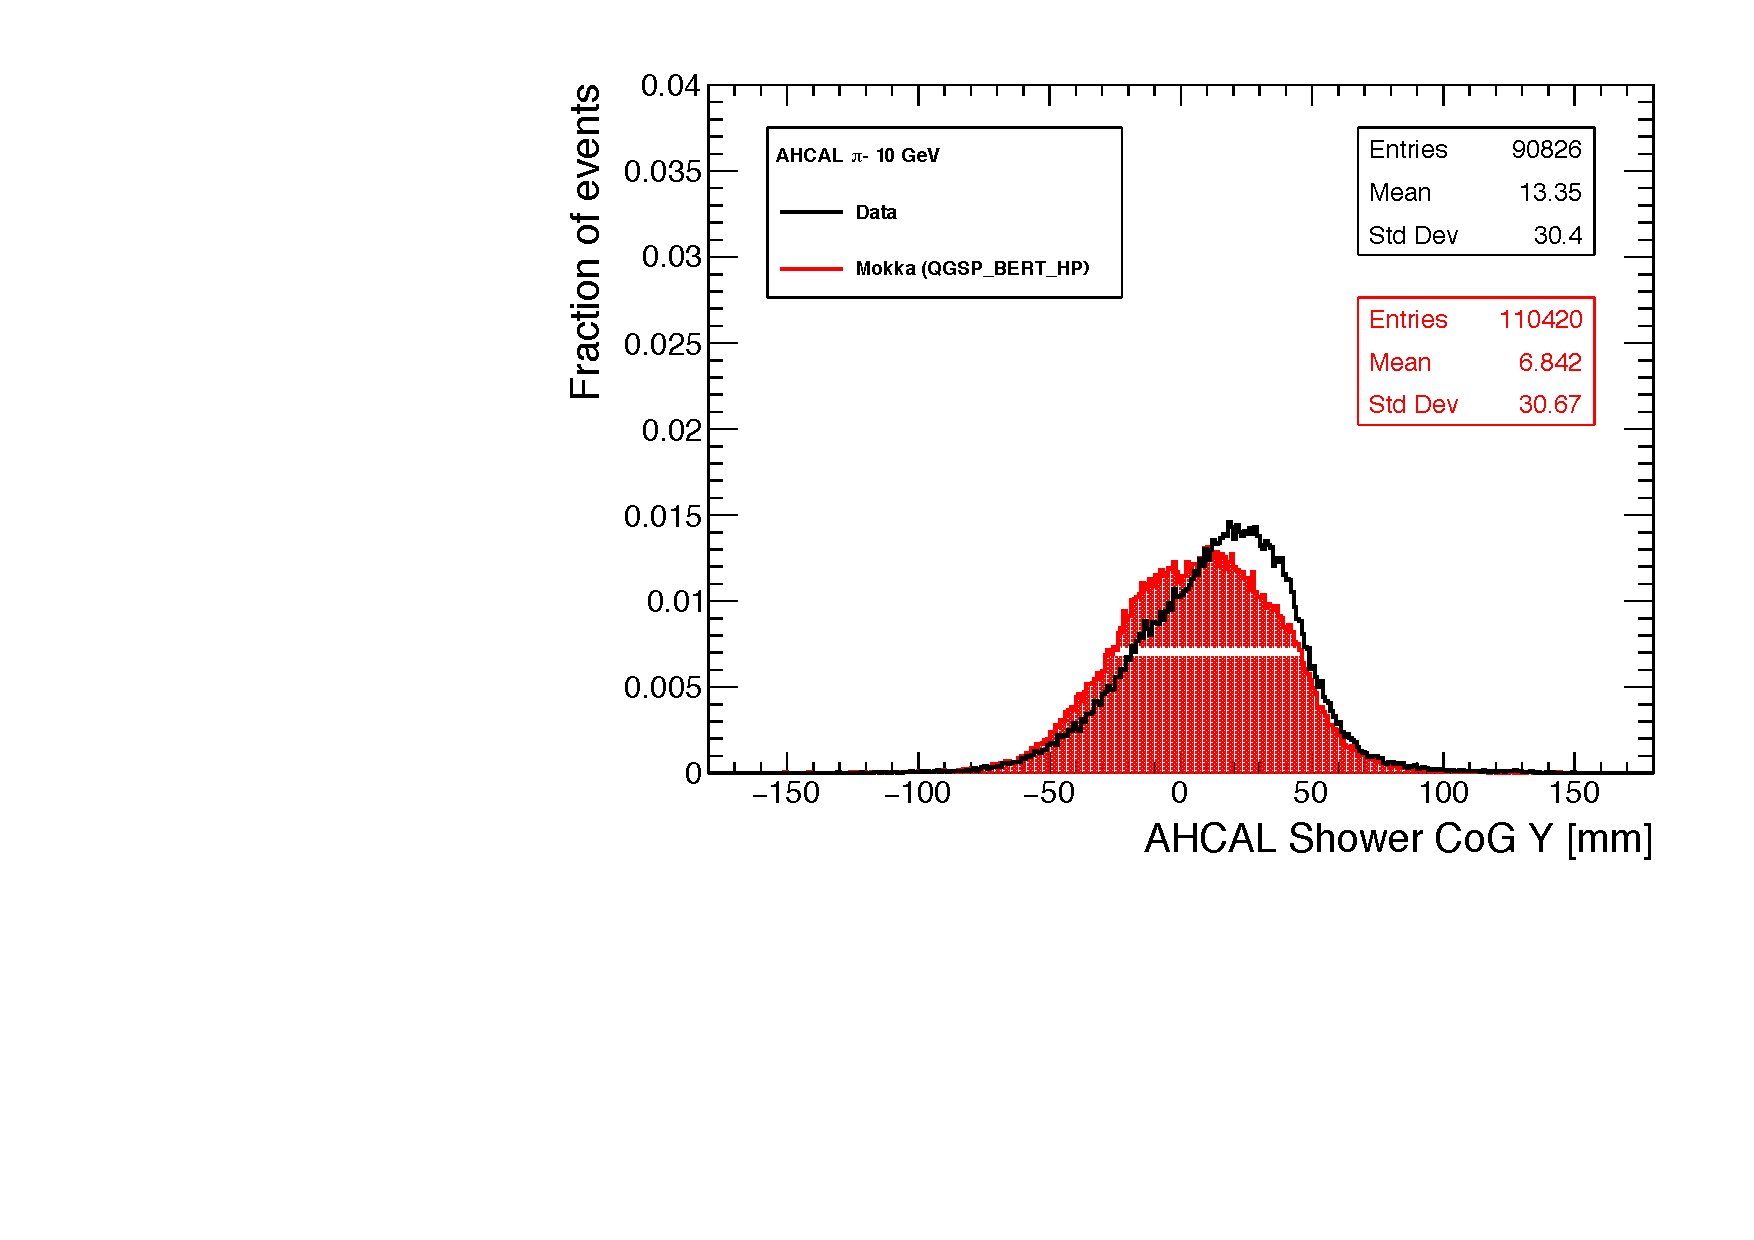
\includegraphics[width=1.\linewidth]{chap5/fig_AHCAL_Timing/Pions/Run24306_CoGY_AHCAL_10GeV_Comparison.pdf}
    \caption{10 GeV.} \label{fig:pi10GeVY}
  \end{subfigure}
  \hfill
  \begin{subfigure}[t]{0.49\textwidth}
    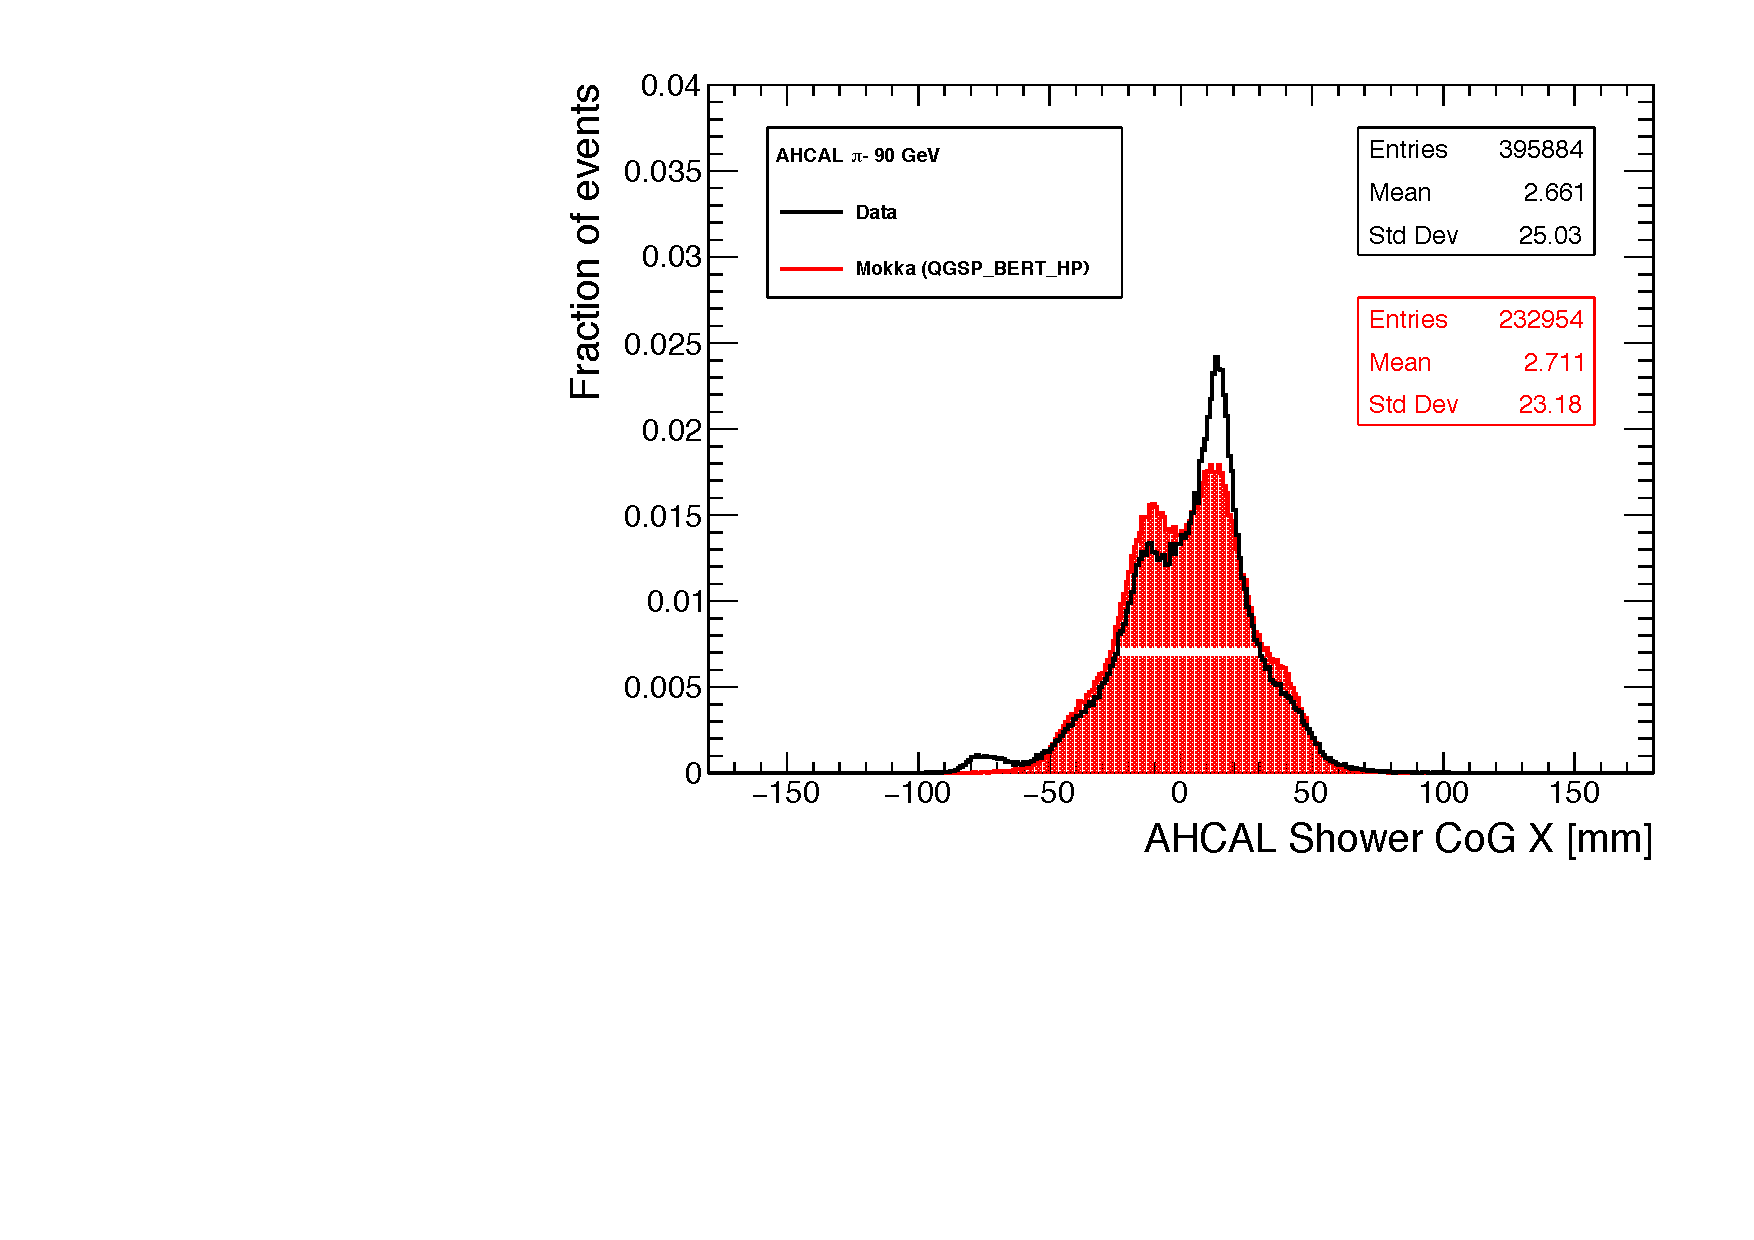
\includegraphics[width=1.\linewidth]{chap5/fig_AHCAL_Timing/Pions/Run24332_CoGX_AHCAL_90GeV_Comparison.pdf}
    \caption{90 GeV.} \label{fig:pi90GeVX}
  \end{subfigure}
  \hfill
  \begin{subfigure}[t]{0.49\textwidth}
    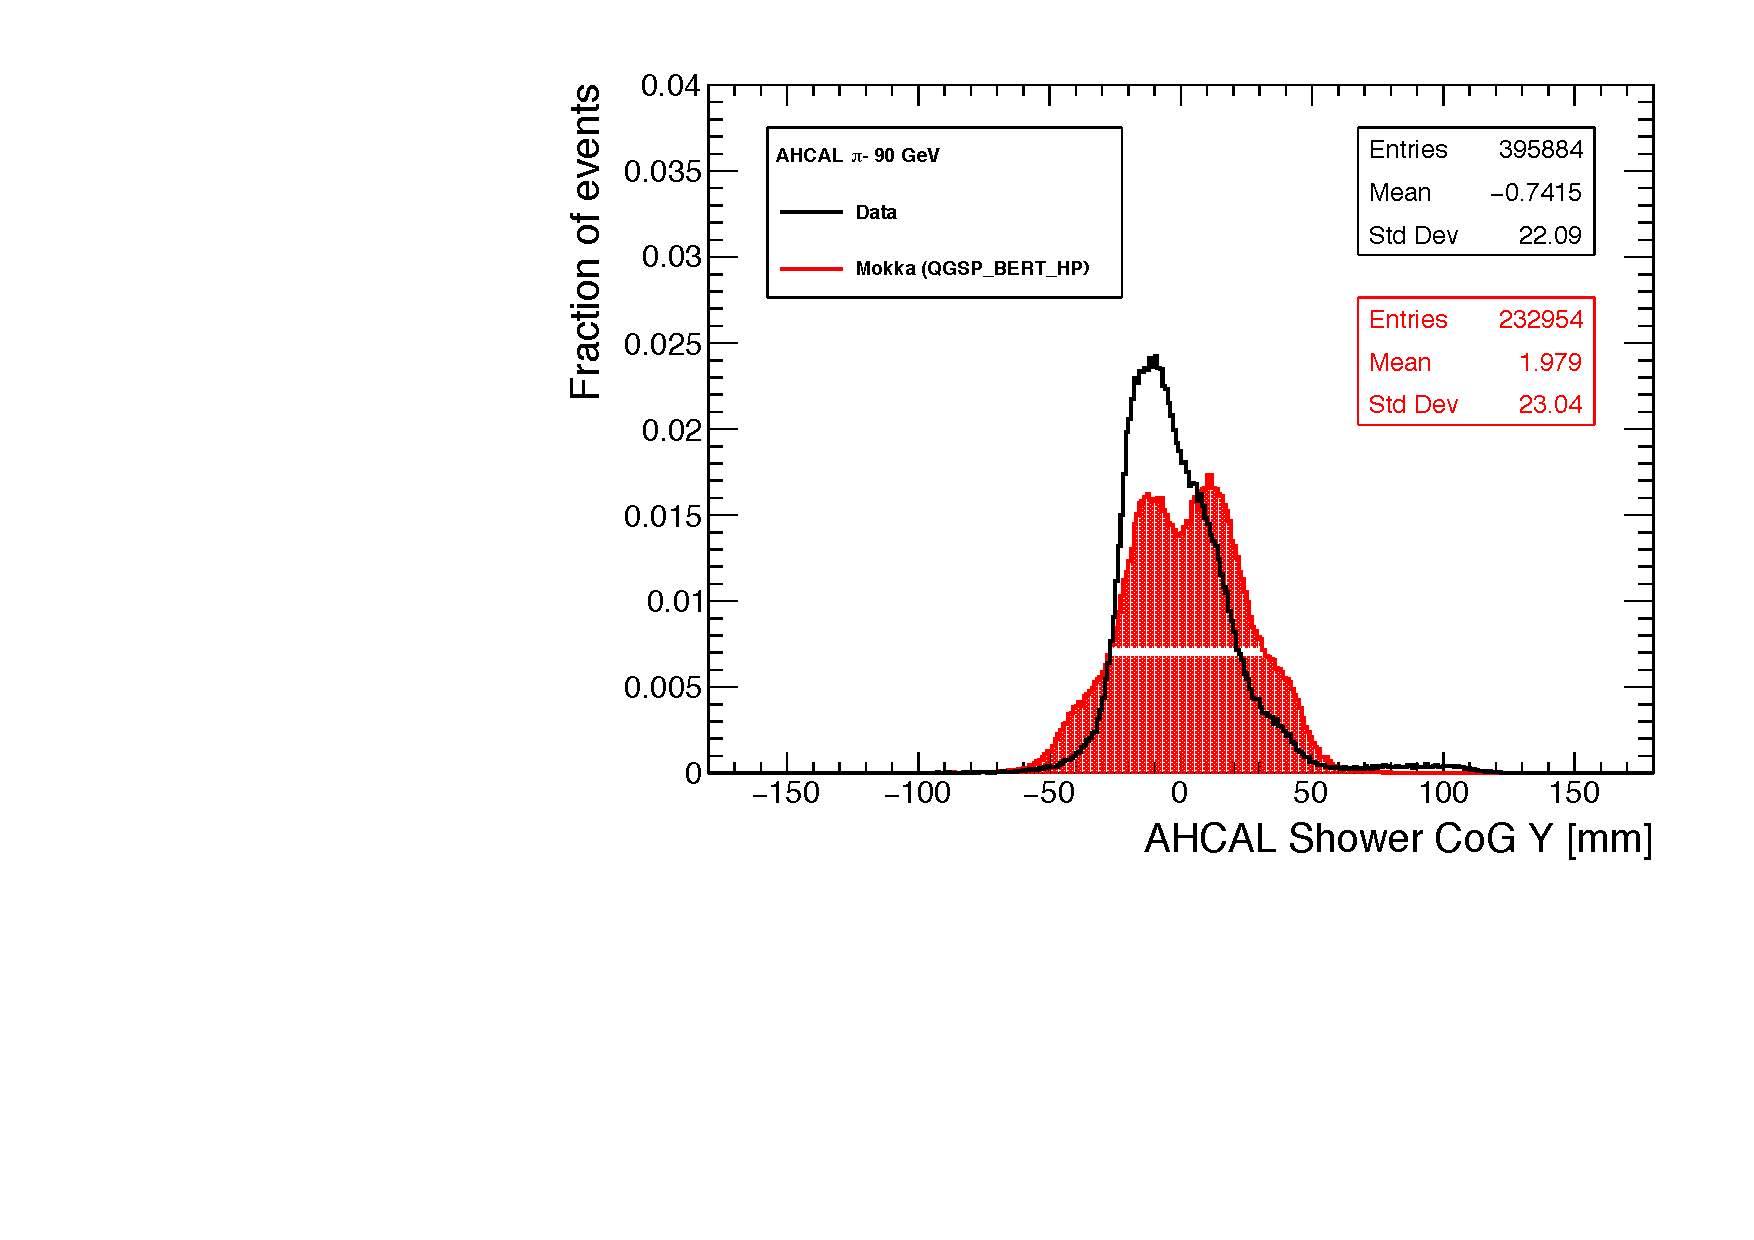
\includegraphics[width=1.\linewidth]{chap5/fig_AHCAL_Timing/Pions/Run24332_CoGY_AHCAL_90GeV_Comparison.pdf}
    \caption{90 GeV.} \label{fig:pi90GeVY}
  \end{subfigure}
  \caption{Beam profiles for 10 GeV and 90 GeV pions for data and simulation in the x and y directions.}
  \label{fig:BPpi}
\end{figure}

\section{Validation of the simulation}

In order to justify any comparison made with the simulation, it needs to be validated first. This is done in two steps using muons and electrons. The comparison of the energy deposited and the number of hits in data and simuation is used to validate the detector simulation. Figures \ref{fig:muVal} show the visible energy $E_{vis}$ and the number of hits above 0.5 MIP for 150 GeV muons in data and simulation.

\begin{figure}[htbp!]
  \centering
  \begin{subfigure}[t]{0.49\textwidth}
    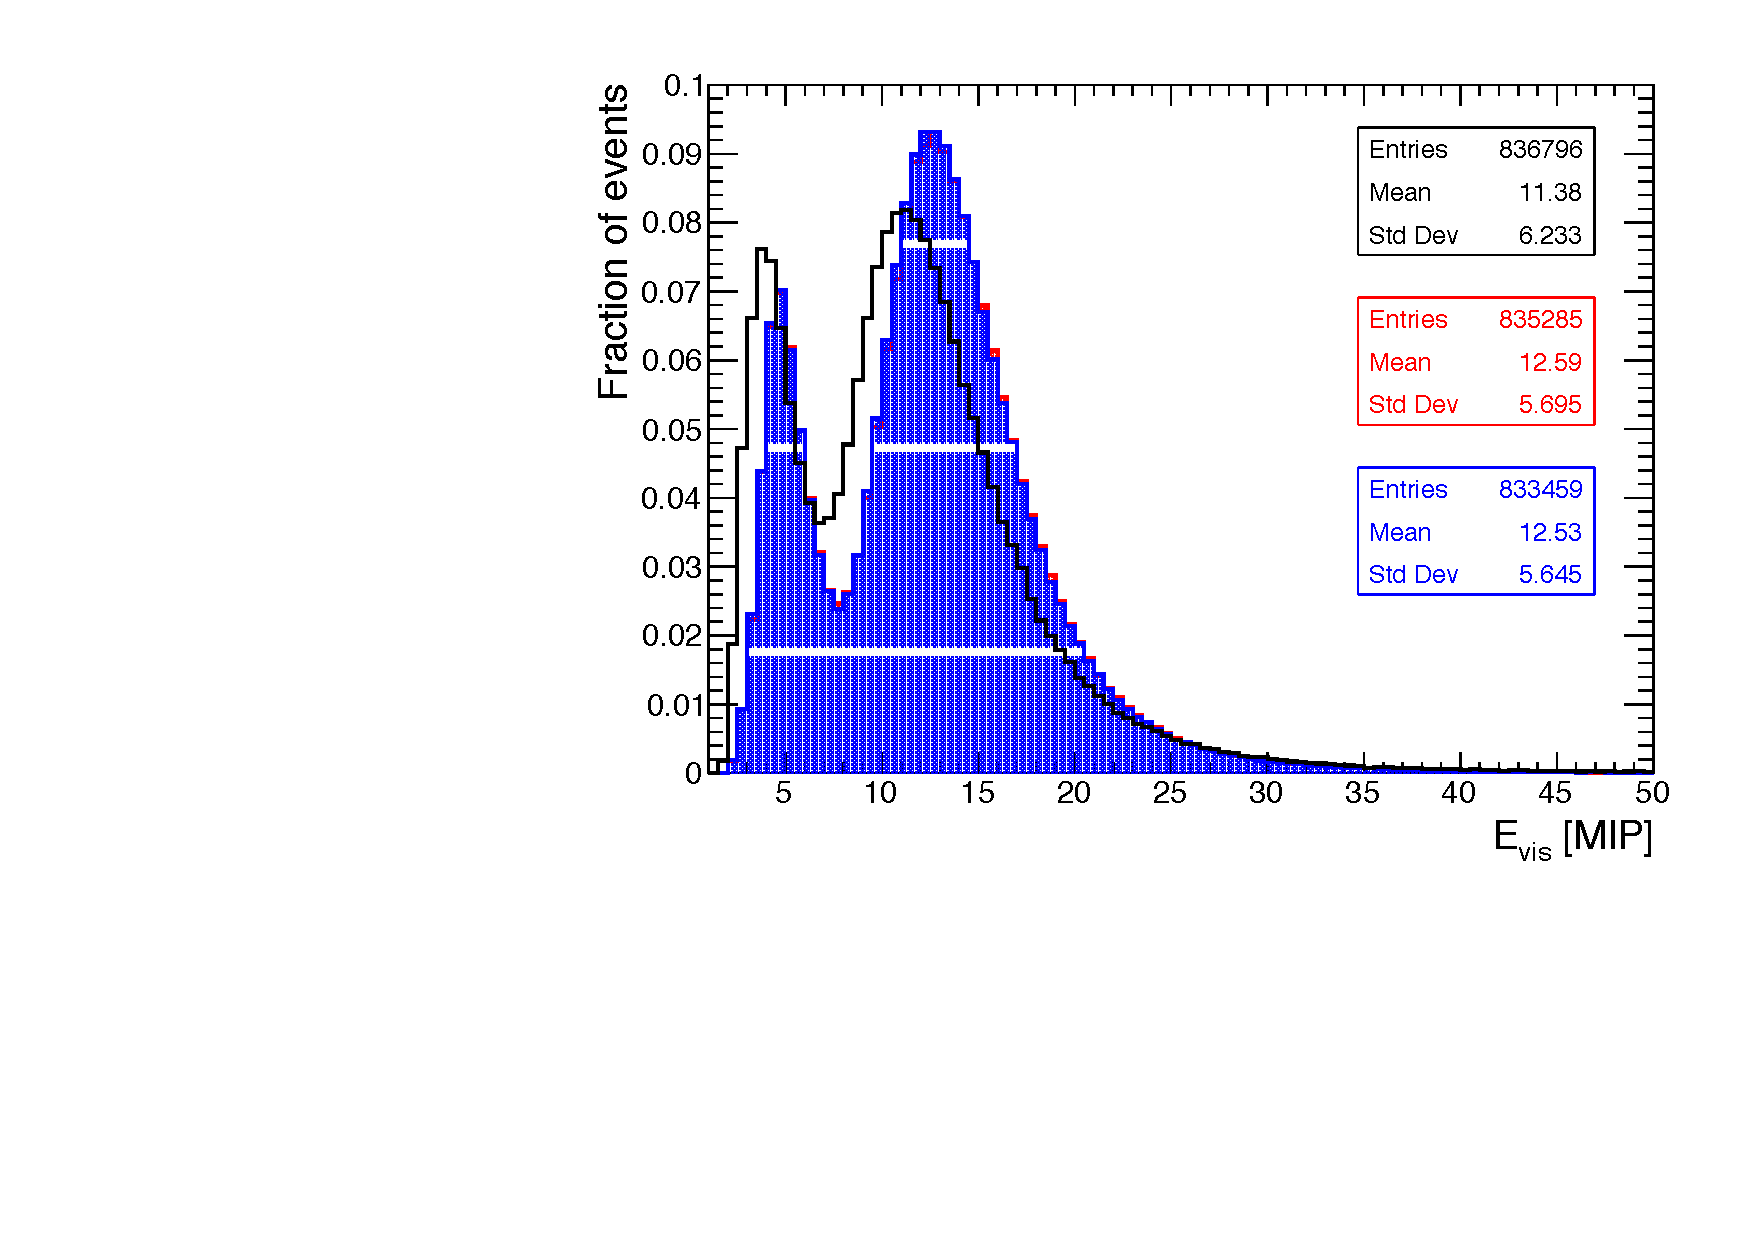
\includegraphics[width=1.\linewidth]{chap5/fig_AHCAL_Timing/Muons/Validation_Evis_Muons.pdf}
    \caption{$E_{vis}$.} \label{fig:muEvis}
  \end{subfigure}
  \hfill
  \begin{subfigure}[t]{0.49\textwidth}
    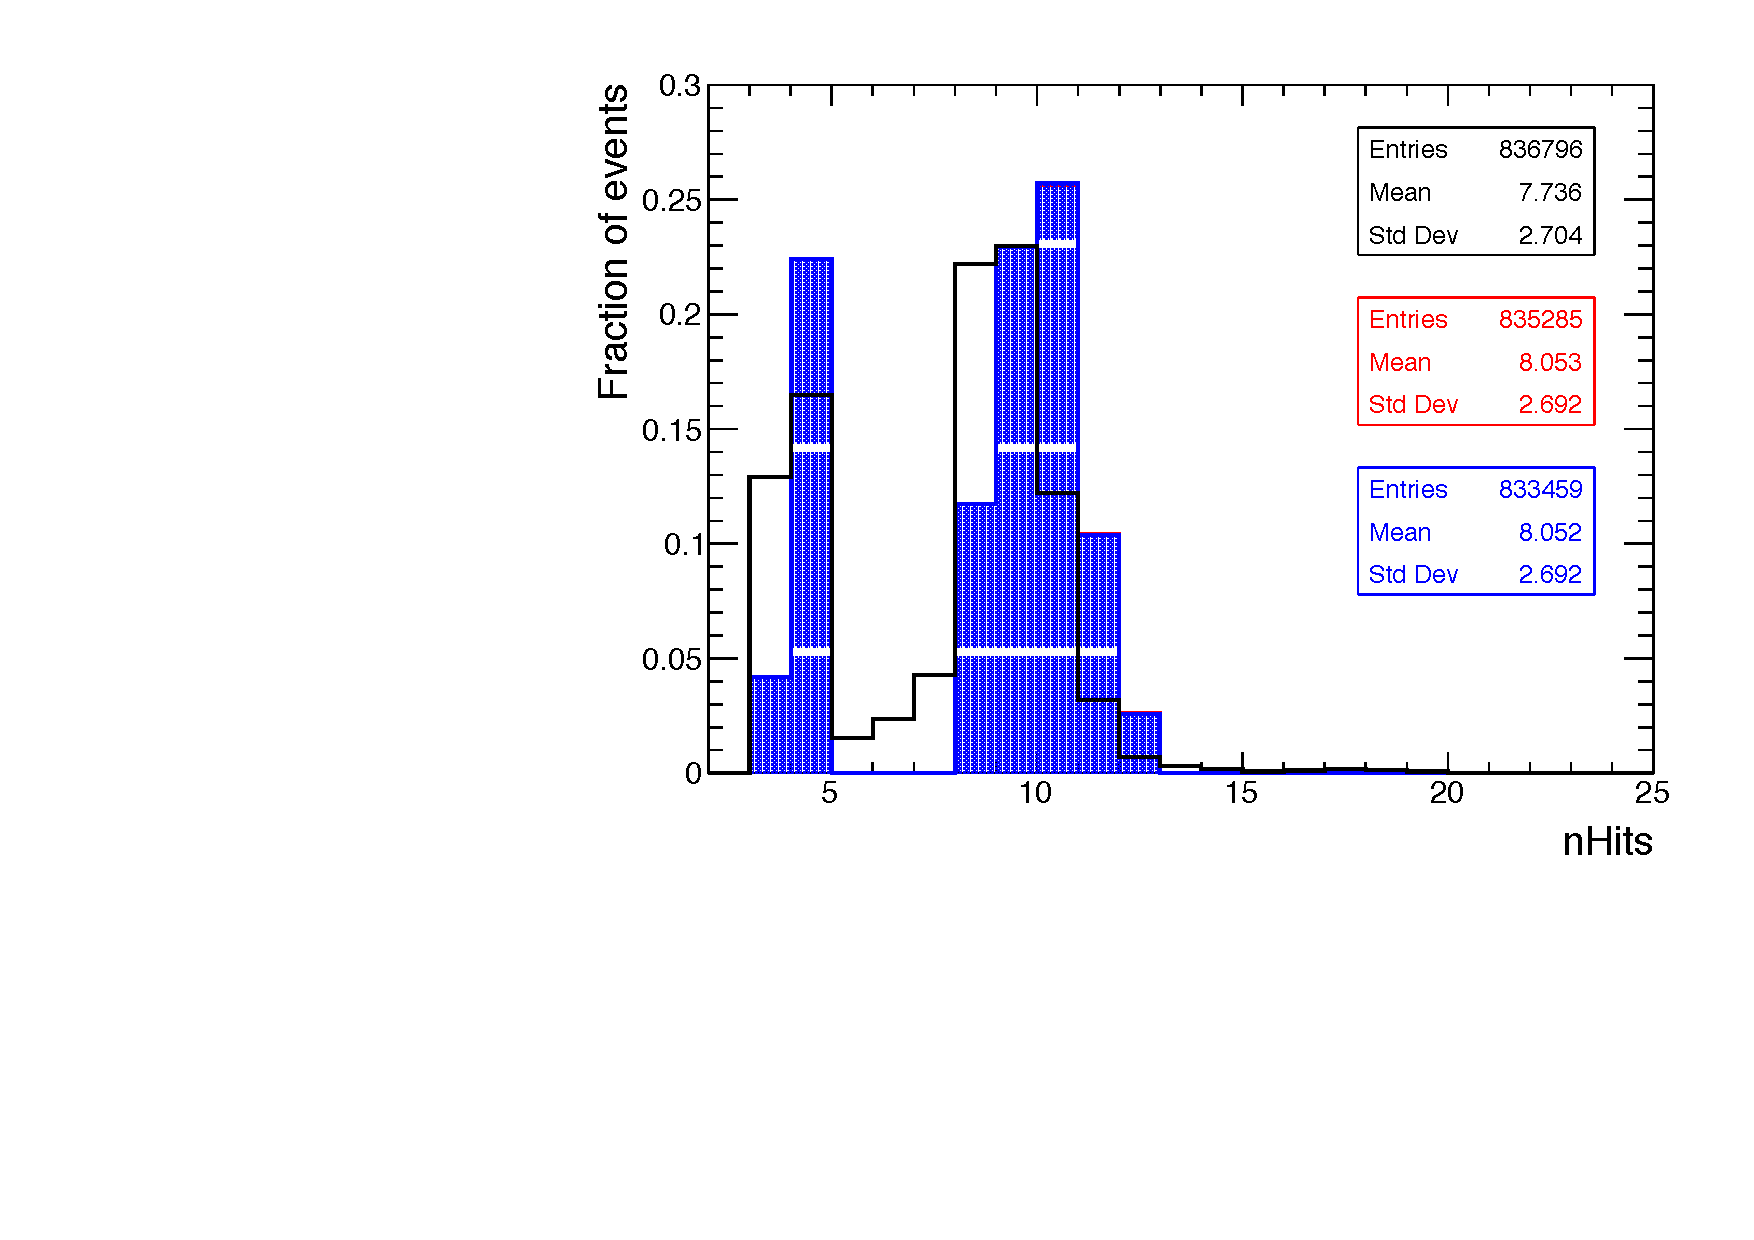
\includegraphics[width=1.\linewidth]{chap5/fig_AHCAL_Timing/Muons/Validation_nHits_Muons.pdf}
    \caption{nHits.} \label{fig:munHits}
  \end{subfigure}
  \caption{\subref{fig:muEvis}) . \subref{fig:munHits}) .}
  \label{fig:muVal}
\end{figure}

One can notice that the distributions are quite similar though the simulation shows a higher mean deposited energy and also less entries to around 5 MIP. As well simulation seems to show a slight higher number of hits. This may be due to the beam profile that is not perfectly well reproduced in simulation. In this case, the impact of dead channels is high depending on where the beam is located. Further, an investigation of the energy deposited per layer has been done and can be seen in figure \ref{fig:muEdep}. It shows that the simulations aggree with data within 5\%. This indicates that the calibration has been performed well for all layers.

\begin{figure}[htbp!]
	\centering
	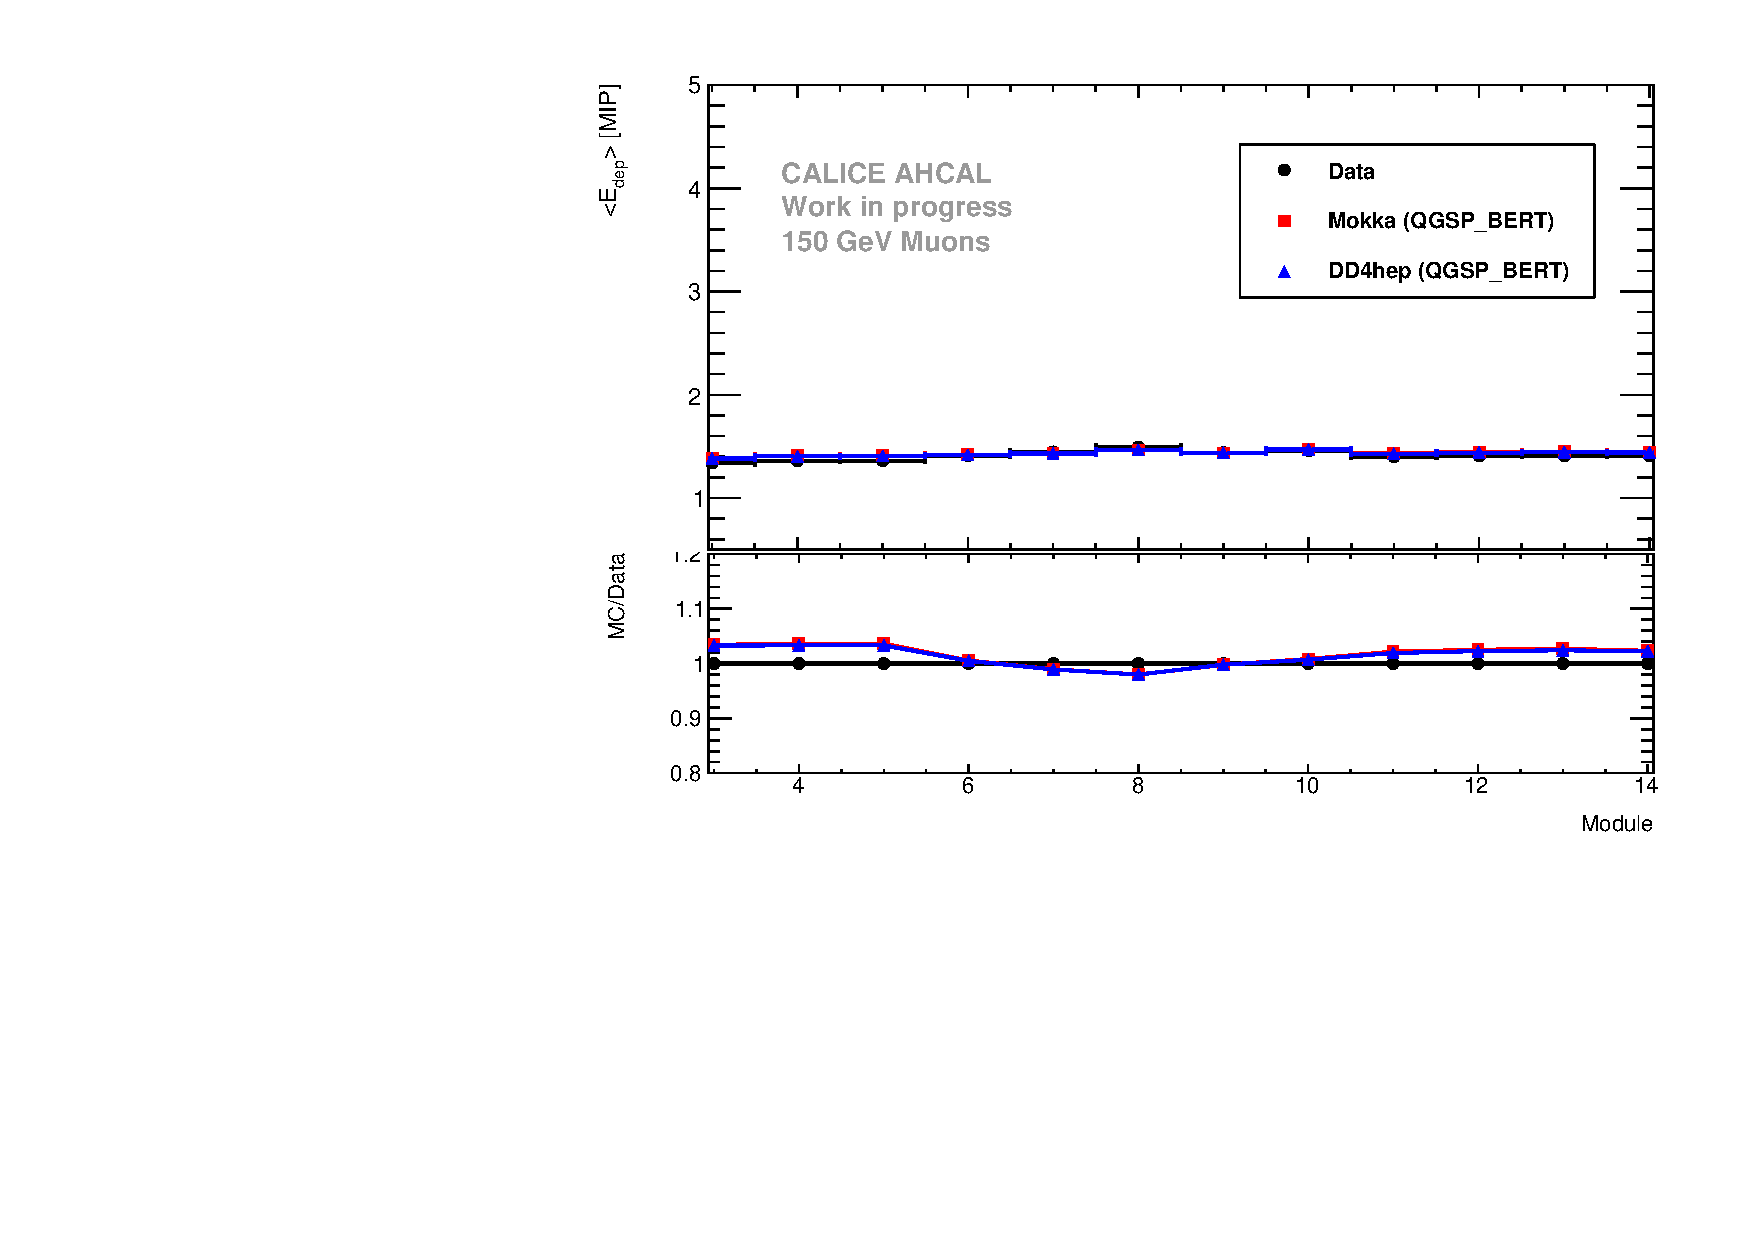
\includegraphics[width=0.7\linewidth]{chap5/fig_AHCAL_timing/Muons/ProfileMuons_Edep.pdf}
	\caption{Mean energy deposited per layer for data and simulation.}
	\label{fig:muEdep}
\end{figure}
